\documentclass[10pt]{article}
\usepackage{graphicx} % Required for inserting images
\usepackage[T1]{fontenc}
\usepackage{float}
\usepackage{amsfonts}
\usepackage{algorithm}
\usepackage{algpseudocode}
\usepackage{amsmath}
\usepackage[a4paper, total={6in, 8in}]{geometry}

\title{ON Lista 4}
\author{Maksymilian Neumann}
\date{Listopad 2023}

\begin{document}

\maketitle

\section{Interpolacja Wielomianowa}
Problem interpolacji wielomianowej formułowany jest następująco: dla danych $n + 1$ par postaci $(x_i, y_i)$, gdzie $x_i \neq x_j$ , mamy za zadanie znaleźć wielomian $p(x)$ jak najniższego stopnia, że $\forall i p(x_i) = y_i$. Na podstawie twierdzenia przedstawionego na wykładzie wiemy, że istnieje dokładnie jeden wielomian stopnia co najwyżej n spełniający ten warunek. W indukcyjnym dowodzie istnienia takiego wielomianu pojawia się wzór
\[p_{k+1}(x) = p_k(x) + c(x - x_0)\dots(x - x_k)\]
dzięki czemu generujemy wielomian wyższego o jeden stopnia zachowując ustalone wartości na poprzednich $x_i$. Postać okazuje się być bardzo przydatna pozwala uniknąć macierzy Vandermond'a która jest słabo uwarunkowana i zmniejszyć złożoność obliczeniową przy wyznaczaniu współczynników.
\[p(x) = \sum_{i=0}^{n+1} c_i \prod_{j=0}^{i-1} (x - x_i)\]
Powyżej tak zwany wzór Newtona do którego będziemy dążyć i z którego będziemy korzystać.

\section{Ilorazy Różnicowe}
Żeby uprościć notacje, wprowadzamy oznaczenie
\[q_i(x) = \prod_{j=0}^{i-1}(x-x_j)\]
mamy $q_0(x)=1$. Wówczas postać Newtona wielomianu p możemy przedstawić jako
\[p(x)=\sum_{i=0}^n c_i q_i(x)\]
p jest rozwiązanie interpolacji, jeżeli spełnia 
\[\forall k \in \{0,\dots,n\} \sum_{i=0}^n c_i q_i (x_k) = y_k\]
Uzyskujemy układ równań
\[A\cdot C = Y\]
gdzie $a_{ij}=q_j(x_i)$, $C = [c_0,\dots,c_n]^T$, a $Y = [y_0,\dots,y_n]^T$. Możemy zobaczyć również że, $\forall i <  j q_j(x_i)=0$, co oznacza że macierz A jest dolnotrójkątna. Umożliwia nam to łatwiejsze znalezienie $c_i$ rozwiązując układ z góry na dół. Łatwo wtedy  zauważyć, że $c_0$ zależy od $y_0 = f(x_0)$, c1 od $y_0$ i $y_1$, itd. Będziemy oznaczać tę zależność jako
\[c_i = f[x_0,\dots,x_i]\]
nazywamy ten czynnik ilorazem różnicowym funkcji $f$ opartym na węzłach $x_0,\dots,x_i$. Wiemy również że ilorazy różnicowe spełniają zależność rekurencyjną
\[f[x_i,\dots,x_k]=\frac{f[x_{i+1},\dots,x_k] - f[x_{i},\dots,x_{k-1}]}{x_k - x_i}\]
gdzie $f[x_i]=y_i$. W najprostszym podejściu do wyznaczania moglibyśmy użyć dwu wymiarowej tablicy $C$, gdzie $C[i,j]=f[x_i,\dots,x_{i+j}]$. Zauważmy jednak, że po wyznaczeniu wszystkich ilorazów opartych na k węzłach, częściowe ilorazy oparte na k - 1 węzłach stają się bezużyteczne (z wyjątkiem $f[x_0,\dots,x_{k-1}]$, który jest jednym z szukanych współczynników) widząc to możemy wnioskować że można zaoszczędzić pamieć potrzebną do rozwiązania.
Rozpoczynamy z wektorem $\hat{d}$ wypełnionym wartościami interpolowanej funkcji w zadanych węzłach. Na wyjściu chcemy dostać wektor ilorazów różnicowych postaci $f[x_0,\dots,x_i]$ będących współczynnikami wielomianu we wzorze Newtona. Zauważmy, że element na pierwszym miejscu w $ \hat{d}$, czyli $d_0$, jest już odpowiedniej postaci. Reszta elementów jest za to postaci $f[x_i]$, możemy zatem wyznaczyć z ich pomocą wszystkie ilorazy zależne od dwóch węzłów n.p.
\[d'_1 = f[x_0, x_1] = \frac{f[x_1] - f[x_0]}{x_1 - x_0} = \frac{d_1 - d_0}{x_1 - x_0}\]
Zauważmy również, że po wyznaczeniu $f[x_{n-1},x_1]$ nie użyjemy już do niczego ilorazu $f[x_n]$, możemy zatem nadpisać go tą nową wartością, tymczasem na przykład $f[x_1]$ potrzebny będzie jeszcze do wyznaczenia $f[x_1, x_2]$. Będziemy zatem szli od końca nadpisując $d_i$ po obliczeniu jego nowej wartości. Po jednej takiej rundzie uzyskamy wszystkie ilorazy oparte na dwóch węzłach. Wówczas $d_1 = f[x_0,x_1]$ przyjmie już swoją ostateczną postać. Wykonujemy kolejną rundę, ponownie od końca, tym razem zatrzymując się na wyliczeniu $d_3$. Po n takich rundach nasz wektor wynikowy przyjmie już ostateczną postać.\\\\
$\hat{x}$ - wektor węzłów , $\hat{y}$ - wektor wartości, $n$ - długość wektorów, $\hat{c}$ - wektor ilorazów różnicowych $f[x_0,\dots,x_i]$

\begin{algorithm}[H]
\caption{Ilorazy Różnicowe}\label{alg:cap}
\begin{algorithmic}
    \Function{ilorazyRoznicowe}{$\hat{x}$, $\hat{y}$, $n$}
    \State $\hat{c} \gets \hat{y}$
    \For{$j = 1, \dots, n$}
        \For{$i = n, \dots, j$}
            \State $c_i \gets \frac{c_i - c_{i-1}}{x_i - x_{i-j}}$
        \EndFor
    \EndFor
    \State \Return $\hat{c}$
    \EndFunction
\end{algorithmic}
\end{algorithm}

\section{Uogólniony Schemat Hornera}
Za zadanie mamy teraz wyznaczenie wartości uzyskanego wielomianu postaci Newtona w danym punkcie. Łatwo zauważyć, że standardowa metoda liczenia ”według wzoru” pozwala nam na dokonanie tego z kwadratową złożonością. Okazuje się jednak, że możemy rozłożyć nasz wielomian w sposób, który umożliwi złożoność liniową. Mamy więc
\[p(x) = \sum_{i=1}^n f[x_0,\dots,x_i]q_i(x) = f[x_0] + \sum_{i=1}^n f[x_0,\dots,x_i](x-x_0)\dots(x-x_i) =\]
\[= f[x_0] + (x- x_0)(f[x_0, x_1] + \sum_{i=2}^n f[x_0,\dots,x_i] (x-x_1)\dots(x-x_i) =\dots\]
\[= f[x_0] + (x - x_0)(f[x_0, x_1] + (x - x_1)(\dots(f[x_0,\dots,x_{n-1}] + (x - x_{n-1}) f[x_0,\dots,x_n])\dots))\]
Będziemy zatem obliczać wartość naszego wielomianu ”od środka”, zaczynając od najbardziej zagnieżdżonych elementów. Taka metodologia to zasadniczo schemat Hornera w bazie $\{q_i(x) : 0 \leq i \leq n\}$ zamiast tradycyjnej $\{1, x, \dots,x^n\}$. W sformalizowanej formie:
\begin{center}
    $w_n(x) = f[x_0,\dots,x_n]$\\
    $w_k(x) = f[x_0,\dots,x_k] + (x - x_k)w_{k+1}$ dla $k < n$\\
    $p(x) = w_0(x)$
\end{center}
Można łatwo zobaczyć że w ten sposób możemy wyznaczyć poszukiwaną wartość z użyciem jednej pętli t.j. w czasie liniowym.\\\\
$\hat{x}$ - wektor węzłów, $n$ - długość wektorów, $\hat{c}$ - wektor ilorazów różnicowych $f[x_0,\dots,x_i]$, $t$ - w którym należy obliczyć wartość wielomianu, $v$ - wartość wielomianu w punkcie t

\begin{algorithm}[H]
\caption{Uogólniony Schemat Hornera}\label{alg:cap}
\begin{algorithmic}
    \Function{warNewton}{$\hat{x}$, $\hat{c}$, $n$, $t$}
    \State $v \gets c_n$
    \For{$i = n-1, \dots, 0$}
        \State $v \gets c_i + (t - x_i)\cdot v$
    \EndFor
    \State \Return $v$
    \EndFunction
\end{algorithmic}
\end{algorithm}

\section{Postać Naturalna}
Postacią naturalną wielomianu nazywamy jego przedstawienie w bazie $\{1, x, x2, x3, \dots\}$, to znaczy
\[p(x) = \sum_{i=0}^n a_ix^i\]
Celem oszczędności znaków, przyjmiemy z powrotem oznaczenie $c_i=f[x_0,\dots,x_i]$. Pierwszym spostrzeżeniem potrzebnym nam do rozwiązania problemu jest fakt, że $a_n$ - współczynnik przy $x^n$ - jest równy $c_n$. Spróbujemy teraz przeżyć kilka pierwszych iteracji algorytmu Hornera z poprzedniej sekcji, skupiając się na współczynnikach przy konkretnych potęgach.
\[w_{n-1} = c_{n-1} + (x - x_{n-1})w_n\]
skąd otrzymujemy pierwsze składowe współczynnika przy $x^{n-1} : c_{n-1}$ i $ -x_{n-1}c_n$. Pójdźmy krok dalej
\[w_{n-2} = c_{n-2} + (x - x_{n2})w_{n-1}\]
Tutaj sytuacja trochę się zmienia, bo $w_{n-1}$, w odróżnieniu od $w_n$, jest wielomianem stopnia większego niż 0. Przyjrzyjmy się dokładniej drugiemu składnikowi tej sumy, rozbijając go na dwie części:
\[x\cdot w_{x-1} = \underbrace{x^2c_n}_{a_n} + \underbrace{x(c_{n-1} - x_{n-1}c_n)}_{\text{”stare” $a_{n-1}$}}\]
\[-x_{n-2}\cdot w_{n-1} = \underbrace{-x_{n-2}c_n\cdot x}_{\text{"nowe" do $a_{n-1}$}} - \underbrace{x_{n-2}(c_{n-1} - x_{n-1}c_n)}_{\text{część startowego $a_{n-2}$}} \]
Sprawdźmy co się stanie w 3 iteracji
\[x\cdot w_{x-2} = \underbrace{x^3c_n}_{a_n} + \underbrace{x^2(c_{n-1} - (x_{n-1}+x_{n-2}) c_n)}_{\text{"nowsze stare" $a_{n-1}$}} + \underbrace{x(c_{n-2} - x_{n-2}(c_{n-1} - x_{n-1} c_n))}_{\text{"stare" $a_{n-2}$}}\]
\[ -x_{n-3}\cdot w_{n-2} = \underbrace{ -x_{n-3} c_n x^2 }_{\text{"nowe" do $a_{n-1}$}} + \underbrace{ -x_{n-3} ( c_{n-1} - ( x_{n-1} + x_{n-2} ) c_n ) }_{\text{"nowe" do $a_{n-2}$}} + \underbrace{ -x_{n-3} ( c_{n-2} - x_{n-2} ( c_{n-1} - x_{n-1} c_n ) ) }_{\text{część startowego $a_{n-3}$}} \]

Okazuje się zatem, że w każdej iteracji (cofając się jak w algorytmie Hornera, poza pierwszą) wyznaczamy bazową wartość przy obecnej potędze (dla $x^i$ będzie to $c_i - x_ia_{i+1}$), a następnie musimy jeszcze zaktualizować współczynniki przy wyższych potęgach o "nowo odkryty" składnik. Z powyższych rozważań można zauważyć, że do każdego aj, że $i < j < n$ dodajemy w i - tej iteracji składnik postaci $-x_{n-i}a_{j+1}$, gdzie $a_{j+1}$ odpowiada obecnemu stanowi naszej wiedzy (widać to w przykładach - ”nowe” części dla $a_{n-1}$ i $a_{n-2}$). Zaprojektujemy zatem algorytm oparty o dokładnie taką technikę. Jego złożoność jest kwadratowa, ponieważ dla każdego kroku ”odwinięcia” (kroku algorytmu Hornera) musimy zaktualizować wszystkie współczynniki dla wyższych potęg.\\\\
$\hat{x}$ - wektor węzłów, $n$ - długość wektorów, $\hat{c}$ - wektor ilorazów różnicowych $f[x_0,\dots,x_i]$, $\hat{a}$ - wektor współczynników wielomianu w postaci naturalnej

\begin{algorithm}[H]
\caption{Postać Naturalna}\label{alg:cap}
\begin{algorithmic}
    \Function{naturalna}{$\hat{x}$, $\hat{c}$, $n$}
    \State $a_n \gets c_n$
    \For{$i = n-1, \dots, 0$}
        \State $a_i \gets c_i - x_i \cdot a_{i+1}$
        \For{$j = i+1, \dots , n-1$}
            \State $a_j \gets a_j - x_i \cdot a_{j+1}$
        \EndFor
    \EndFor
    \State \Return $\hat{a}$
    \EndFunction
\end{algorithmic}
\end{algorithm}

\section{Wykresy}
Za zadanie mamy połączenie naszych implementacji w jedną funkcje umożliwiającą graficzne porównacie wynikowego wielomianu z interpolowaną funkcją. Robimy to przez podzielenie danego przez użytkownika przedziału $[a,b]$ na $n+1$ równoległych węzłów i obliczamy dla ich wartości funkcji. Następnym krokiem jest wyznaczenie ilorazów różnicowych dzięki którym będziemy mogli ustalić wartość wielomianu w punkcie. Dyskretyzujemy przedział w taki sposób, żeby móc
ujrzeć wartości wielomianu także poza węzłami ( najlepiej $N\cdot (n+1)$ punktów na przedziale $[a,b]$, gdzie $N>1$ całkowite, wtedy wśród nich znajdą się nasze węzły).Dla każdego z punktów obliczamy wartość funkcji i wielomianu, a następnie uzyskane wyniki umieszczamy na wykresie.\\\\
$f$ - interpolowana funkcja, $[a, b]$ - przedział interpolacji, $n$ - stopień wielomianu

\begin{algorithm}[H]
\caption{Generator Wykresów}\label{alg:cap}
\begin{algorithmic}
    \Function{rysujNnfx}{$f$, $a$, $b$, $n$}
    \State $h \gets \frac{b-a}{n}$
    \For{$k = 0, \dots, n$}
        \State $x_k \gets a + k\cdot h$
        \State $y_k \gets f(x_k)$
    \EndFor
    \State $\hat{c} \gets ilorazyRoznicowe(\hat{x}, \hat{y})$
    \State $pt \gets N \cdot (n+1)$
    \State $dx \gets \frac{b-a}{pt - 1}$
    \For{$i = 0,\dots, pt$}
        \State $X_i \gets sa + i \cdot dx$
        \State $W_i = warNewton(\hat{x}, \hat{c}, X_i)$
        \State $F_i = f(X_i)$
    \EndFor
    \State $plot(x=\Hat{H}, y=[\Hat{W}, \Hat{F}] )$
    \EndFunction
\end{algorithmic}
\end{algorithm}


\section{Zadanie 5}
\subsection{Opis problemu}
Za zadanie mamy użycie zaimplementowanych funkcji na przykładach:
\begin{enumerate}
    \item $f(x) = e^x$ na przedziale $[0, 1]$
    \item $f(x) = x^2 \cdot sin(x)$ na przedziale $[-1, 1]$
\end{enumerate}
Dla wielomianów stopni $n = 5,10,15$
\subsection{Rozwiązanie}
Zadanie zostało rozwiązane za pomocą funkcji opisanych w tym dokumencie zaimplementowanych w języku Julia.
\subsection{Wyniki}
Możemy zaobserwować, że obie testowane funkcje dają się bardzo dokładnie interpolować, to znaczy dla obu wartości wielomianów interpolacyjnych dowolnego ze sprawdzanych stopni niemal pokrywają się z wartościami funkcji na całym zadanym przedziale.
\begin{center}
    \Huge{Funkcja 1}
\end{center}
\begin{figure}[H]
    \centering
    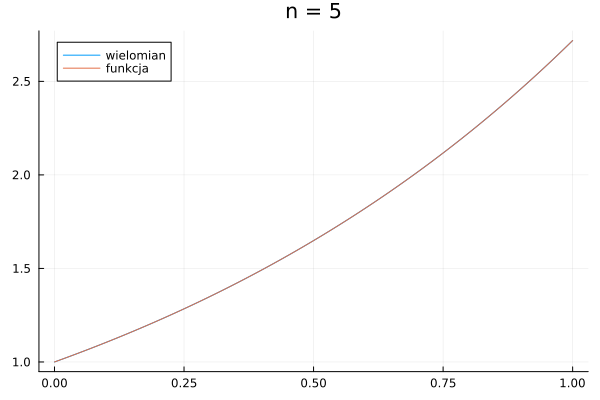
\includegraphics[width=0.6\linewidth]{z5f1_5.png}
    \label{fig:enter-label}
\end{figure}
\begin{figure}[H]
    \centering
    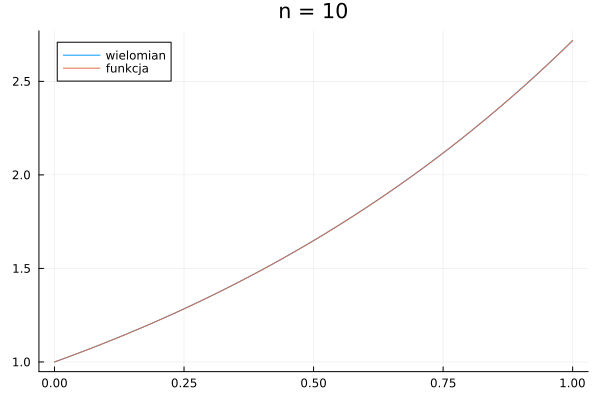
\includegraphics[width=0.6\linewidth]{z5f1_10.png}
    \label{fig:enter-label}
\end{figure}
\begin{figure}[H]
    \centering
    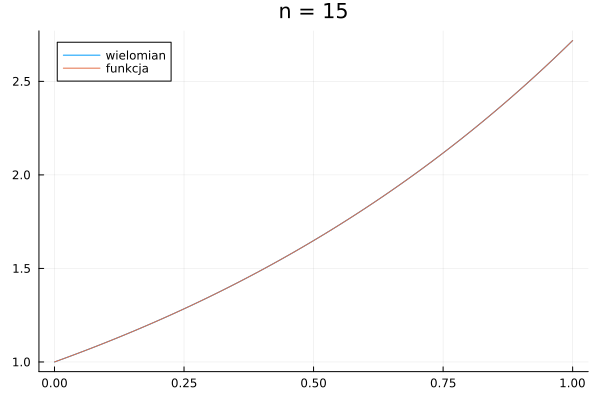
\includegraphics[width=0.6\linewidth]{z5f1_15.png}
    \label{fig:enter-label}
\end{figure}
\begin{center}
    \Huge{Funkcja 2}
\end{center}
\begin{figure}[H]
    \centering
    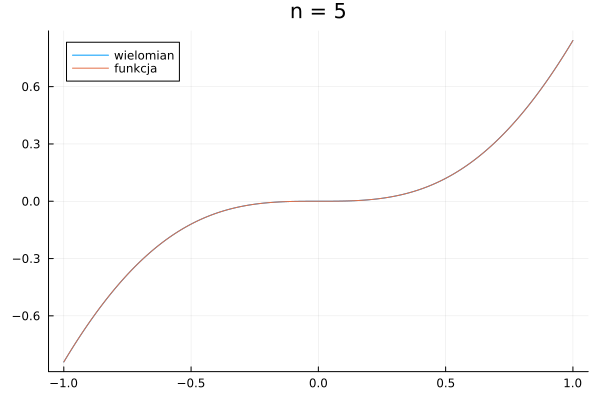
\includegraphics[width=0.6\linewidth]{z5f2_5.png}
    \label{fig:enter-label}
\end{figure}
\begin{figure}[H]
    \centering
    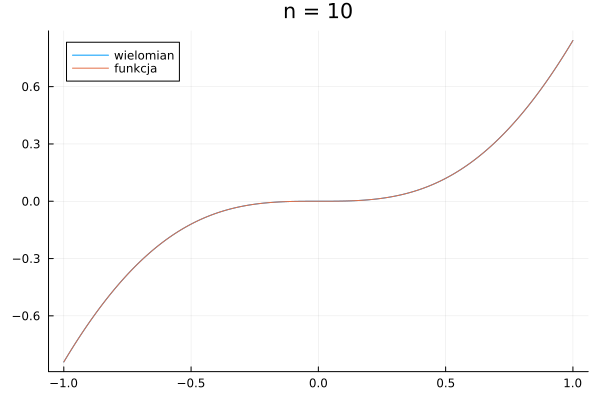
\includegraphics[width=0.6\linewidth]{z5f2_10.png}
    \label{fig:enter-label}
\end{figure}
\begin{figure}[H]
    \centering
    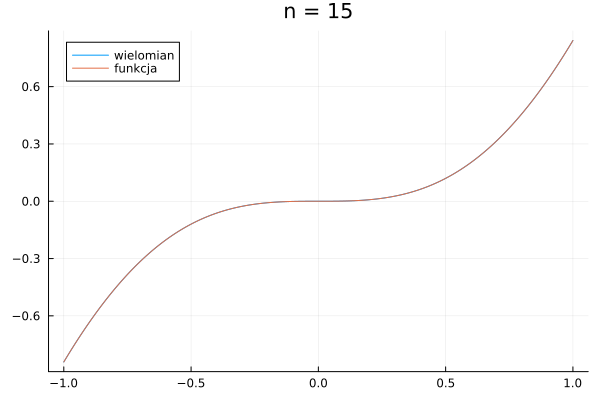
\includegraphics[width=0.6\linewidth]{z5f2_15.png}
    \label{fig:enter-label}
\end{figure}
\section{Zadanie 6}
\subsection{Opis problemu}
Zadanie to jest analogiczne do poprzedniego aczkolwiek na funkcjach:
\begin{enumerate}
    \item $f(x) = |x|$ na przedziale $[-1, 1]$
    \item $f(x) = \frac{1}{1+x^2}$ na przedziale $[-5, 5]$
\end{enumerate}
Dla wielomianów stopni $n = 5,10,15$
\subsection{Rozwiązanie}
Zadanie zostało rozwiązane za pomocą funkcji opisanych w tym dokumencie zaimplementowanych w języku Julia.
\subsection{Wyniki}
W przeciwieństwie do poprzedniego zadania, tym razem funkcje nie interpolują się za dobrze. Co więcej, wzrost
stopnia wielomianu nie niesie za sobą poprawy dokładności.\\
W przypadku funkcji $|x|$ problemem jest jej nieróżniczkowalność. Intuicyjnie można powiedzieć, że wielomiany są raczej okrągłe, dlatego wierzchołek wykresu stanowi dla nich trudność.\\
Dla funkcji $\frac{1}{1+x^2}$ obserwujemy zjawisko Rungego, które polega na zwiększaniu się rozbieżności na końcach przedziału wraz ze zwiększaniem stopnia wielomianu interpolacyjnego. Pojawia się ono, gdy węzły interpolacji są równoodległe, co ma miejsce w przypadku naszej implementacji. Rozwiązaniem tego problemu mógłby być na przykład dobór punktów w taki sposób, żeby na przy krańcach przedziału występowało ich większe zagęszczenie.\\

\begin{center}
    \Huge{Funkcja 1}
\end{center}
\begin{figure}[H]
    \centering
    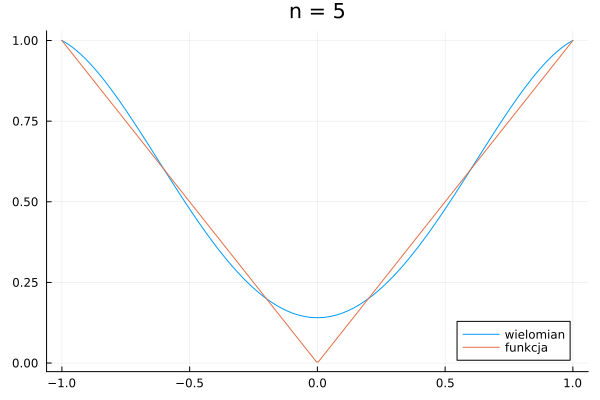
\includegraphics[width=0.6\linewidth]{z6f1_5.png}
    \label{fig:enter-label}
\end{figure}
\begin{figure}[H]
    \centering
    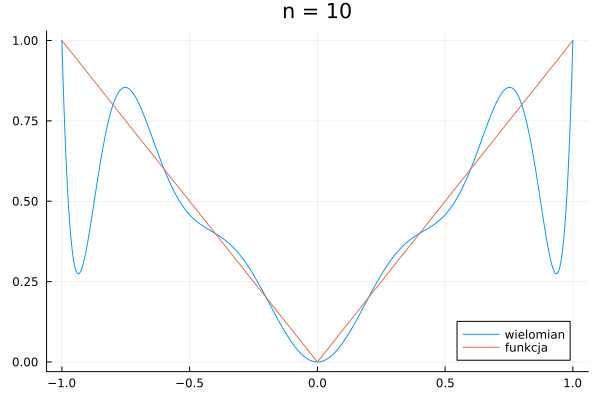
\includegraphics[width=0.6\linewidth]{z6f1_10.png}
    \label{fig:enter-label}
\end{figure}
\begin{figure}[H]
    \centering
    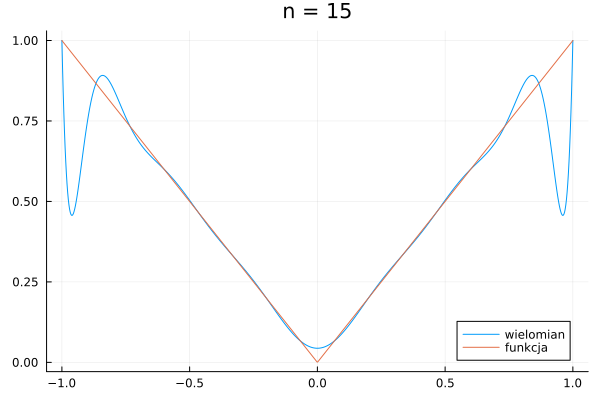
\includegraphics[width=0.6\linewidth]{z6f1_15.png}
    \label{fig:enter-label}
\end{figure}
\begin{center}
    \Huge{Funkcja 2}
\end{center}
\begin{figure}[H]
    \centering
    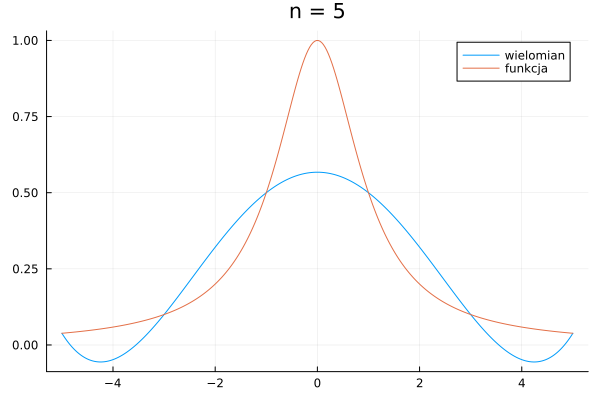
\includegraphics[width=0.6\linewidth]{z6f2_5.png}
    \label{fig:enter-label}
\end{figure}
\begin{figure}[H]
    \centering
    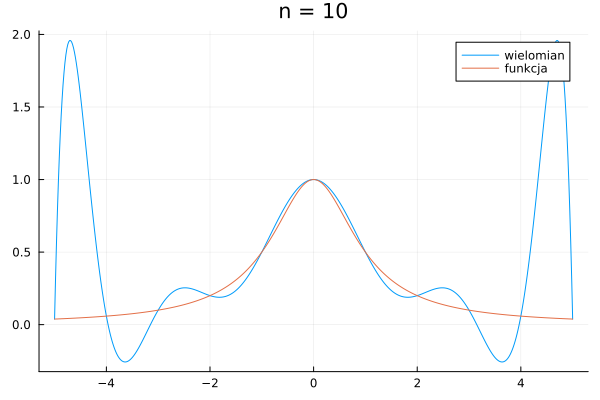
\includegraphics[width=0.6\linewidth]{z6f2_10.png}
    \label{fig:enter-label}
\end{figure}
\begin{figure}[H]
    \centering
    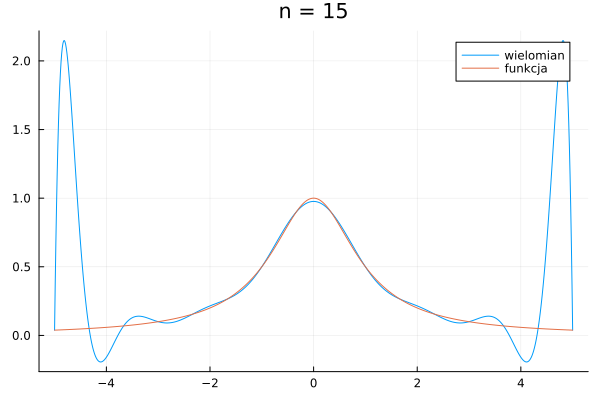
\includegraphics[width=0.6\linewidth]{z6f2_15.png}
    \label{fig:enter-label}
\end{figure}

\section{Wnioski}
Interpolacja wielomianowa jest dosyć dobrą metodą przybliżania funkcji, gdy znamy jej wartości tylko w niektórych punktach, ale trzeba pamiętać o jej ograniczeniach. Świetnie radzi sobie z gładkimi, zaokrąglonymi funkcjami jak te z zadania 5. Taka intuicja może być jednak zgubna – druga funkcja z zadania 6 również może wydawać się bardzo porządna, a jednak natrafiliśmy na trudności. Należy mieć na uwadze, że bezmyślne zwiększanie stopnia wielomianu może przynieść więcej szkody niż pożytku. W niektórych przypadkach bardziej pomocne może okazać się z kolei przemyślane rozstawienie węzłów interpolacji. Narysowanie wykresu może dać nam pewną intuicję w kwestii tego rozstawu.

\end{document}
